% \documentclass[aspectratio=169, 11pt]{beamer}
\documentclass[aspectratio=169, 11pt, handout]{beamer}
 
% ── Theme ──
\usetheme{Madrid}
\usecolortheme{default}
\setbeamertemplate{navigation symbols}{}
\setbeamertemplate{footline}{%
  \leavevmode\hbox{%
    \begin{beamercolorbox}[wd=.333333\paperwidth,ht=2.5ex,dp=1ex,center]{author in head/foot}%
      \usebeamerfont{author in head/foot}\insertshortauthor
    \end{beamercolorbox}%
    \begin{beamercolorbox}[wd=.333333\paperwidth,ht=2.5ex,dp=1ex,center]{title in head/foot}%
      \usebeamerfont{title in head/foot}\insertshorttitle
    \end{beamercolorbox}%
    \begin{beamercolorbox}[wd=.333333\paperwidth,ht=2.5ex,dp=1ex,right]{date in head/foot}%
      \usebeamerfont{date in head/foot}\insertframenumber{} / \inserttotalframenumber\hspace*{2ex}
    \end{beamercolorbox}}}
 
% ── Packages ──
\usepackage{amsmath,amssymb}
\usepackage{booktabs}
\usepackage{xcolor}
\usepackage{colortbl}
\usepackage{tikz}
\usetikzlibrary{arrows.meta, positioning}
\usetikzlibrary{calc}
 
% ── Colors ──
\definecolor{sbgreen}{HTML}{00704A}
\definecolor{warnred}{HTML}{CC0000}
\definecolor{noteblue}{HTML}{2060A0}
 
% ── Commands ──
\newcommand{\E}{\mathbb{E}}
\newcommand{\Var}{\mathrm{Var}}
\newcommand{\Cov}{\mathrm{Cov}}
\newcommand{\SE}{\mathrm{SE}}
\newcommand{\Prob}{\mathrm{Pr}}
\newcommand{\indep}{\perp\!\!\!\perp}
\DeclareMathOperator{\plim}{plim}
 
% ── Reusable TikZ styles ──
\tikzset{
    tnode/.style={draw, rounded corners, fill=gray!10, minimum width=2.2cm, minimum height=0.65cm, font=\small, align=center},
    tgreen/.style={tnode, fill=sbgreen!15, draw=sbgreen},
    tblue/.style={tnode, fill=noteblue!12, draw=noteblue},
    tred/.style={tnode, fill=red!8, draw=warnred},
    tarrow/.style={-{Stealth}, thick}
}

% ── Title ──
\title[Lecture 5]{Lecture 5: Causal Forests}
\subtitle{Applied ML for Business Part II}
\author{Zhikun Lu}
\date{\today}

\begin{document}

% ====================================================================
\begin{frame}
\titlepage
\end{frame}

% ====================================================================
\begin{frame}{Where We Are}

\begin{center}
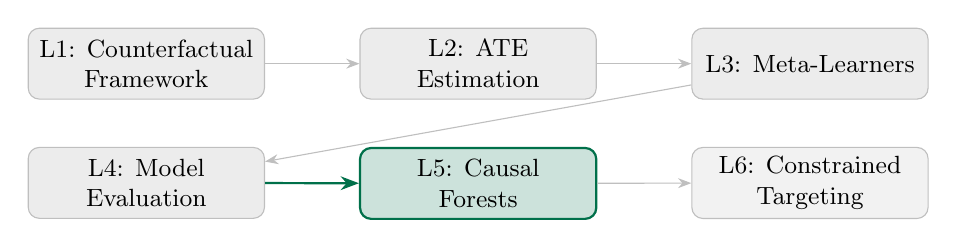
\begin{tikzpicture}[
    node distance=0.6cm and 1.2cm,
    box/.style={draw, rounded corners, minimum width=3cm, minimum height=0.9cm, font=\small, align=center},
    done/.style={box, fill=gray!15, draw=gray!50},
    active/.style={box, fill=sbgreen!20, draw=sbgreen, thick},
    inactive/.style={box, fill=gray!10, draw=gray!50}
]
\node[done] (L1) {L1: Counterfactual\\Framework};
\node[done, right=of L1] (L2) {L2: ATE\\Estimation};
\node[done, right=of L2] (L3) {L3: Meta-Learners};
\node[done, below=of L1] (L4) {L4: Model\\Evaluation};
\node[active, below=of L2] (L5) {L5: Causal\\Forests};
\node[inactive, below=of L3] (L6) {L6: Constrained\\Targeting};

\draw[-{Stealth}, gray!50] (L1) -- (L2);
\draw[-{Stealth}, gray!50] (L2) -- (L3);
\draw[-{Stealth}, gray!50] (L3) -- (L4);
\draw[-{Stealth}, thick, sbgreen] (L4) -- (L5);
\draw[-{Stealth}, gray!50] (L5) -- (L6);
\end{tikzpicture}
\end{center}
\end{frame}

% ====================================================================
\begin{frame}{Today's Plan}

\textbf{Causal Forests: Directly Targeting $\tau(x)$}
\begin{enumerate}
    \item Decision trees: splitting on outcome heterogeneity
    \item Causal trees: splitting on treatment effect heterogeneity
    \item From trees to forests; statistical inference
    \item Generalized random forests
\end{enumerate}

\bigskip

\textbf{Next time (Lecture 6):} Constrained Targeting.

\end{frame}

% ====================================================================
\begin{frame}{Running Example: Starbucks Coupon Campaign}
 
Two features: \textbf{customer type} (exec/analyst) and \textbf{spending history} (high/low).

Coupon ($D$) randomly assigned with probability $e = 0.5$.
 
\bigskip
 
\begin{center}
\begin{tabular}{llcccc}
\toprule
\textbf{Type} & \textbf{Spending} & \textbf{Share} & $\E[Y(1) \mid X]$ & $\E[Y(0) \mid X]$ & $\tau(x)$\\
\midrule
Executive & High & 25\% & 0.65 & 0.60 & $+0.05$ \\
Executive & Low  & 25\% & 0.35 & 0.30 & $+0.05$ \\
Analyst   & High & 25\% & 0.50 & 0.30 & $+0.20$ \\
Analyst   & Low  & 25\% & 0.20 & 0.00 & $+0.20$ \\
\bottomrule
\end{tabular}
\end{center}
 
\pause
\bigskip
 
\textbf{Spending history} is purely prognostic: it shifts $Y$ by $\pm 0.15$, but $\tau$ is the same across high/low.
 
\textbf{Customer type} is the effect modifier: $\tau(\text{analyst}) = 0.20 \neq 0.05 = \tau(\text{exec})$.
 
\end{frame}
 
 
% %%%%%%%%%%%%%%%%%%%%%%%%%%%%%%%%%%%%%%%%%%%%%%%%%%%%%%%%%%%%%%%%%%%%
\section{Why Outcome-Based Methods Fail}
% %%%%%%%%%%%%%%%%%%%%%%%%%%%%%%%%%%%%%%%%%%%%%%%%%%%%%%%%%%%%%%%%%%%%
 
% ====================================================================
\begin{frame}{Review: How a Decision Tree Works}
 
A decision tree partitions the covariate space into leaves and predicts $\hat{Y}_\ell = \bar{Y}_\ell$ in each leaf.
 
\bigskip
 
\textbf{Splitting criterion:} choose the split that maximizes the between-group variance:
\[
\Delta_{\text{CART}}(\text{split}) = \frac{n_L}{n_P}(\bar{Y}_L - \bar{Y}_P)^2 + \frac{n_R}{n_P}(\bar{Y}_R - \bar{Y}_P)^2
\]
 
The split that creates the biggest gap in $\bar{Y}$ wins.
 
\pause
\bigskip
 
\textbf{Regularization} (minimum leaf size, maximum depth, pruning) limits the number of splits.
 
Each split must explain enough outcome variance to justify the added complexity. Variables with small outcome gaps are pruned first.
 
\end{frame}
 
% ====================================================================
\begin{frame}{The Outcome Variance Hierarchy}
 
Pool treated and control. Rank candidate splits by outcome gap:
 
\bigskip
 
\begin{center}
\begin{tabular}{lccc}
\toprule
\textbf{Candidate split} & \textbf{Gap in $\bar{Y}$} & \textbf{Gap in $\tau$} & \textbf{Rank by $\bar{Y}$} \\
\midrule
Spending history & $|0.5125 - 0.2125| = \mathbf{0.30}$ & $|0.125 - 0.125| = 0$ & 1st \\
Customer type & $|0.475 - 0.25| = 0.225$ & $|0.05 - 0.20| = \mathbf{0.15}$ & 2nd \\
Coupon $D$ & $|0.425 - 0.30| = 0.125$ & --- & 3rd \\
\bottomrule
\end{tabular}
\end{center}
 
\pause
\bigskip
 
The prognostic variable dominates. The effect modifier comes second. The treatment itself comes last.
 
Under regularization, the coupon effect (0.125) will be pruned before spending (0.30) and type (0.225).
 
\end{frame}
 
% ====================================================================
\begin{frame}{S-Learner under Strong Regularization}
 
The S-Learner fits $\hat{\mu}(X, D)$ jointly. With strong regularization, max depth = 1. The coupon $D$ competes for splits against spending and type.
 
\bigskip
 
\begin{center}
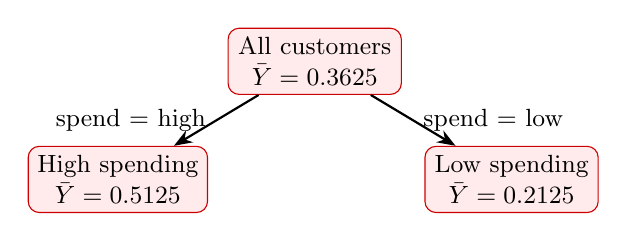
\begin{tikzpicture}
\node[tred] (root) at (0, 2.2) {All customers\\ $\bar{Y} = 0.3625$};
\node[tred] (l) at (-2.5, 0.7) {High spending\\ $\bar{Y} = 0.5125$};
\node[tred] (r) at (2.5, 0.7) {Low spending\\ $\bar{Y} = 0.2125$};
\draw[tarrow] (root) -- (l) node[midway, left, font=\small]{spend = high};
\draw[tarrow] (root) -- (r) node[midway, right, font=\small]{spend = low};
\end{tikzpicture}
\end{center}
 
\bigskip

Spending wins the first split (gap 0.30).
 
\medskip

\pause 

Coupon $D$ never enters. $\hat{\tau}(x) = \hat{\mu}(x, 1) - \hat{\mu}(x, 0) = 0$ for everyone.
 
\end{frame}
 
 
 
% ====================================================================
\begin{frame}{S-Learner under Moderate Regularization}
 
Allow two splits. After spending, the next largest gap is customer type (0.225), which still beats coupon (0.125).
 
\bigskip
 
\begin{center}
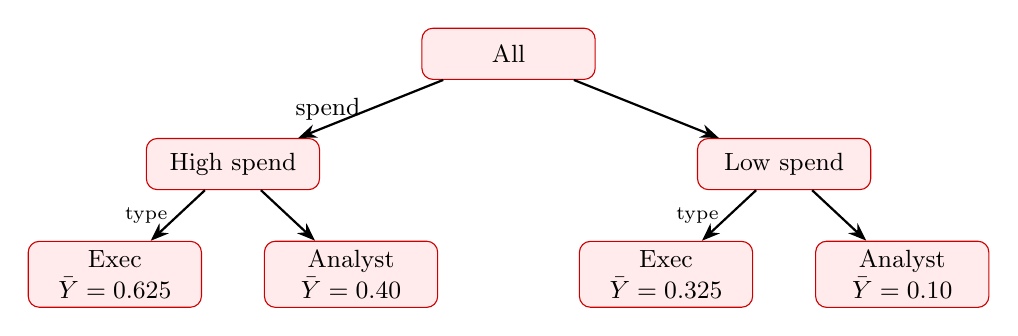
\begin{tikzpicture}[level distance=1.4cm, sibling distance=2.8cm]
\node[tred] (root) at (0, 2.8) {All};
\node[tred] (l) at (-3.5, 1.4) {High spend};
\node[tred] (r) at (3.5, 1.4) {Low spend};
\node[tred] (ll) at (-5.0, 0) {Exec\\$\bar{Y}=0.625$};
\node[tred] (lr) at (-2.0, 0) {Analyst\\$\bar{Y}=0.40$};
\node[tred] (rl) at (2.0, 0) {Exec\\$\bar{Y}=0.325$};
\node[tred] (rr) at (5.0, 0) {Analyst\\$\bar{Y}=0.10$};
\draw[tarrow] (root) -- (l) node[midway, left, font=\small]{spend};
\draw[tarrow] (root) -- (r) node[midway, right, font=\small]{};
\draw[tarrow] (l) -- (ll) node[midway, left, font=\scriptsize]{type};
\draw[tarrow] (l) -- (lr) node[midway, right, font=\scriptsize]{};
\draw[tarrow] (r) -- (rl) node[midway, left, font=\scriptsize]{type};
\draw[tarrow] (r) -- (rr) node[midway, right, font=\scriptsize]{};
\end{tikzpicture}
\end{center}
 
\pause
\medskip
 
Coupon \emph{still} never enters. Still $\hat{\tau}(x) = 0$ for everyone.
 
The S-Learner needs \textbf{three} levels of depth (spending $\to$ type $\to$ coupon) to detect any treatment effect at all.
 
\end{frame}
 
% ====================================================================
\begin{frame}{T-Learner under Regularization}
 
The T-Learner fits separate models $\hat{\mu}_1(x)$ and $\hat{\mu}_0(x)$, then subtracts.
 
\bigskip
 
\begin{center}
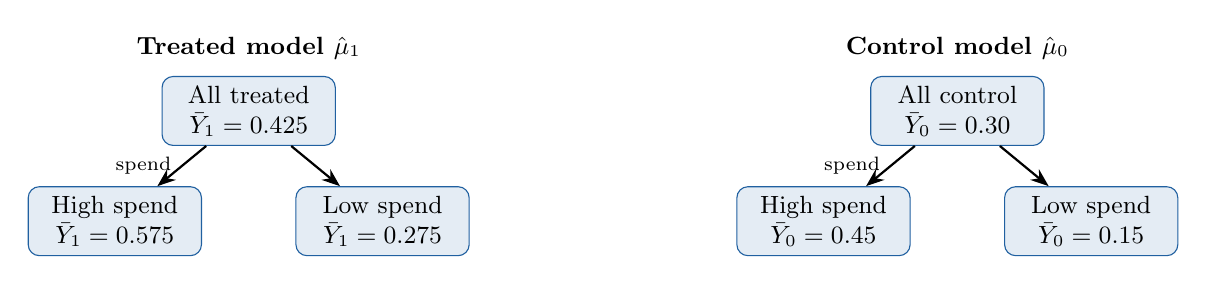
\begin{tikzpicture}
% Treated
\node[font=\small\bfseries] at (-4.5, 2.8) {Treated model $\hat{\mu}_1$};
\node[tblue] (t1) at (-4.5, 2.0) {All treated\\ $\bar{Y}_1 = 0.425$};
\node[tblue] (t1l) at (-6.2, 0.6) {High spend\\$\bar{Y}_1 = 0.575$};
\node[tblue] (t1r) at (-2.8, 0.6) {Low spend\\$\bar{Y}_1 = 0.275$};
\draw[tarrow] (t1) -- (t1l) node[midway, left, font=\scriptsize]{spend};
\draw[tarrow] (t1) -- (t1r);
 
% Control
\node[font=\small\bfseries] at (4.5, 2.8) {Control model $\hat{\mu}_0$};
\node[tblue] (t0) at (4.5, 2.0) {All control\\ $\bar{Y}_0 = 0.30$};
\node[tblue] (t0l) at (2.8, 0.6) {High spend\\$\bar{Y}_0 = 0.45$};
\node[tblue] (t0r) at (6.2, 0.6) {Low spend\\$\bar{Y}_0 = 0.15$};
\draw[tarrow] (t0) -- (t0l) node[midway, left, font=\scriptsize]{spend};
\draw[tarrow] (t0) -- (t0r);
\end{tikzpicture}
\end{center}
 
\pause
\bigskip
 
Both models split on spending (gap 0.30 beats type gap 0.15 in treated arm). Subtract:
\[
\hat{\tau}(\text{high}) = 0.575 - 0.45 = 0.125, \qquad \hat{\tau}(\text{low}) = 0.275 - 0.15 = 0.125
\]
 
\textcolor{warnred}{Constant $\hat{\tau}$ everywhere.} Heterogeneity by customer type completely missed.
 
\end{frame}
 
% ====================================================================
\begin{frame}{Why Prognostic Splits Waste Capacity}
 
The T-Learner's spending split explains a 0.30 gap in each arm.

\bigskip
 
But this gap \emph{cancels} in the subtraction $\hat{\mu}_1 - \hat{\mu}_0$:
\[
0.575 - 0.45 = 0.125 \quad = \quad 0.275 - 0.15 = 0.125
\]
 
\pause
\bigskip
 
The split used all of the model's capacity on a variable that is irrelevant for treatment effects.
 
\bigskip
 
Meanwhile, customer type drives a 0.15 gap in $\tau$ (analyst: 0.20 vs.\ exec: 0.05) but only a 0.15 gap in $Y$ within the treated arm. Under regularization, it loses to spending.
 
\pause
\bigskip
 
\begin{alertblock}{Core Problem}
Both the S-Learner and T-Learner select splits based on \emph{outcome} variation. Variables that predict $Y$ but not $\tau$ consume model capacity and crowd out the variables that matter for targeting.
\end{alertblock}
 
\end{frame}
 
% ====================================================================
\begin{frame}{Effect Modifiers vs.\ Prognostic Variables}
 
\textbf{Effect modifier:} $X_j$ such that $\tau(x)$ varies with $X_j$.
\begin{itemize}
    \item Customer type: $\tau(\text{analyst}) = 0.20 \neq 0.05 = \tau(\text{exec})$
\end{itemize}
 
\bigskip
 
\textbf{Prognostic variable:} $X_j$ that predicts $\E[Y \mid X]$ but not $\tau$.
\begin{itemize}
    \item Spending history: shifts $Y$ by $\pm 0.15$, zero gap in $\tau$
\end{itemize}
 
\pause
\bigskip
 
\begin{center}
\begin{tabular}{lcc}
\toprule
& \textbf{Effect modifier} & \textbf{Prognostic only} \\
\midrule
Useful for targeting? & \textcolor{sbgreen}{Yes} & \textcolor{warnred}{No} \\
Dominates regularized S-Learner? & \textcolor{warnred}{No} & \textcolor{warnred}{Yes} \\
Dominates regularized T-Learner? & \textcolor{warnred}{No} & \textcolor{warnred}{Yes} \\
Dominates Causal Tree? & \textcolor{sbgreen}{Yes} & \textcolor{sbgreen}{No} \\
\bottomrule
\end{tabular}
\end{center}
 
\end{frame}
 
 
% %%%%%%%%%%%%%%%%%%%%%%%%%%%%%%%%%%%%%%%%%%%%%%%%%%%%%%%%%%%%%%%%%%%%
\section{Causal Trees}
% %%%%%%%%%%%%%%%%%%%%%%%%%%%%%%%%%%%%%%%%%%%%%%%%%%%%%%%%%%%%%%%%%%%%
 
% ====================================================================
\begin{frame}{Step 1: The Causal Tree Splitting Criterion}
 
Replace CART's outcome gap with a \emph{treatment effect} gap:
 
\bigskip
 
\begin{block}{Causal Tree Criterion}
At each candidate split of parent $P$ into children $L$ and $R$:
\[
\Delta(\text{split}) = \frac{n_L}{n_P}\bigl(\hat{\tau}_L - \hat{\tau}_P\bigr)^2 + \frac{n_R}{n_P}\bigl(\hat{\tau}_R - \hat{\tau}_P\bigr)^2
\]
where $\hat{\tau}_\ell = \bar{Y}_{1,\ell} - \bar{Y}_{0,\ell}$ is the diff-in-means in leaf $\ell$.
\end{block}
 
\pause
\bigskip
 
A split on a purely prognostic variable produces $\hat{\tau}_L \approx \hat{\tau}_R \approx \hat{\tau}_P$, so $\Delta \approx 0$.
 
The criterion is \emph{blind} to outcome variation that does not translate into treatment effect variation.
 
\end{frame}
 
% ====================================================================
\begin{frame}{Causal Tree: Starbucks Example}
 
Evaluate candidate splits at the root:
 
\bigskip
 
\begin{center}
\begin{tabular}{lcl}
\toprule
\textbf{Candidate split} & $\Delta$ & \textbf{Decision} \\
\midrule
Spending history & $0.5(0.125 - 0.125)^2 + 0.5(0.125 - 0.125)^2 = 0$ & \textcolor{warnred}{$\Delta = 0$} \\
Customer type    & $0.5(0.05 - 0.125)^2 + 0.5(0.20 - 0.125)^2 = 0.0056$ & \textcolor{sbgreen}{Split here!} \\
\bottomrule
\end{tabular}
\end{center}
 
\pause
\bigskip
 
\begin{center}
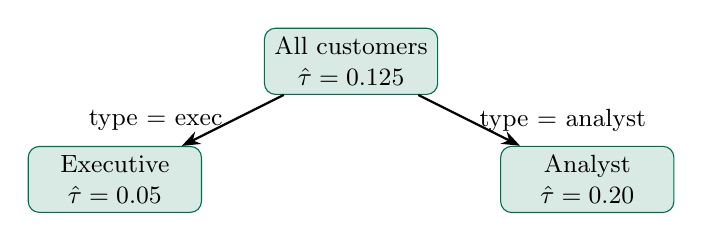
\begin{tikzpicture}
\node[tgreen] (root) at (0, 2.0) {All customers\\ $\hat{\tau} = 0.125$};
\node[tgreen] (l) at (-3.0, 0.5) {Executive\\ $\hat{\tau} = 0.05$};
\node[tgreen] (r) at (3.0, 0.5) {Analyst\\ $\hat{\tau} = 0.20$};
\draw[tarrow] (root) -- (l) node[midway, left, font=\small]{type = exec};
\draw[tarrow] (root) -- (r) node[midway, right, font=\small]{type = analyst};
\end{tikzpicture}
\end{center}
 
\medskip
 
The very first split finds the effect modifier. Under any level of regularization, the causal tree will never waste capacity on a purely prognostic variable.
 
\end{frame}
 
% ====================================================================
\begin{frame}{Side-by-Side: Three Methods Compared}
 
\begin{center}
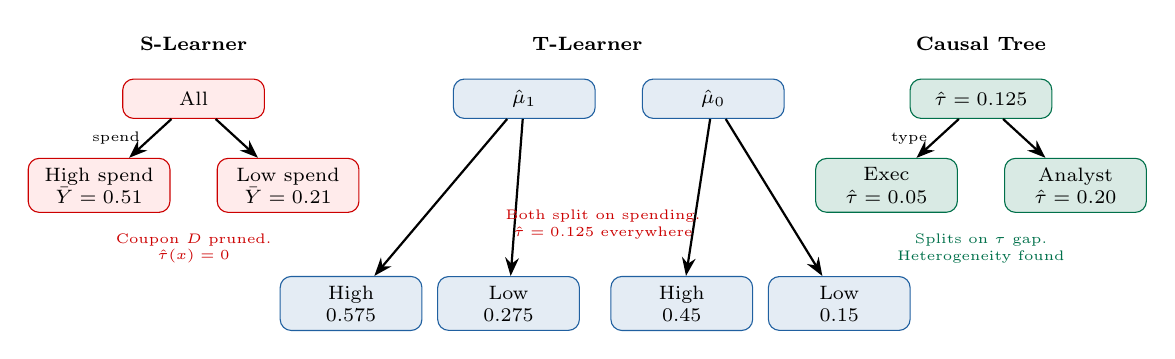
\begin{tikzpicture}[
    snode/.style={draw, rounded corners, minimum width=1.8cm, minimum height=0.5cm, font=\scriptsize, align=center},
    sg/.style={snode, fill=sbgreen!15, draw=sbgreen},
    sb/.style={snode, fill=noteblue!12, draw=noteblue},
    sr/.style={snode, fill=red!8, draw=warnred},
    sarrow/.style={-{Stealth}, thick, font=\tiny}
]
 
% S-Learner
\node[font=\scriptsize\bfseries] at (-5.0, 2.8) {S-Learner};
\node[sr] (s-root) at (-5.0, 2.1) {All};
\node[sr] (s-l) at (-6.2, 1.0) {High spend\\ $\bar{Y}=0.51$};
\node[sr] (s-r) at (-3.8, 1.0) {Low spend\\ $\bar{Y}=0.21$};
\draw[sarrow] (s-root) -- (s-l) node[midway, left]{spend};
\draw[sarrow] (s-root) -- (s-r);
\node[font=\tiny, text=warnred, align=center] at (-5.0, 0.2) {Coupon $D$ pruned.\\$\hat{\tau}(x) = 0$};
 
% T-Learner
\node[font=\scriptsize\bfseries] at (0.0, 2.8) {T-Learner};
\node[sb] (t1) at (-0.8, 2.1) {$\hat{\mu}_1$};
\node[sb] (t1l) at (-3.0, -0.5) {High\\0.575};
\node[sb] (t1r) at (-1.0, -0.5) {Low\\0.275};
\draw[sarrow] (t1) -- (t1l);
\draw[sarrow] (t1) -- (t1r);
\node[sb] (t0) at (1.6, 2.1) {$\hat{\mu}_0$};
\node[sb] (t0l) at (1.2, -0.5) {High\\0.45};
\node[sb] (t0r) at (3.2, -0.5) {Low\\0.15};
\draw[sarrow] (t0) -- (t0l);
\draw[sarrow] (t0) -- (t0r);
\node[font=\tiny, text=warnred, align=center] at (0.2, 0.5) {Both split on spending.\\$\hat{\tau}=0.125$ everywhere};
 
% Causal Tree
\node[font=\scriptsize\bfseries] at (5.0, 2.8) {Causal Tree};
\node[sg] (ct-root) at (5.0, 2.1) {$\hat{\tau} = 0.125$};
\node[sg] (ct-l) at (3.8, 1.0) {Exec\\$\hat{\tau}=0.05$};
\node[sg] (ct-r) at (6.2, 1.0) {Analyst\\$\hat{\tau}=0.20$};
\draw[sarrow] (ct-root) -- (ct-l) node[midway, left]{type};
\draw[sarrow] (ct-root) -- (ct-r);
\node[font=\tiny, text=sbgreen, align=center] at (5.0, 0.2) {Splits on $\tau$ gap.\\Heterogeneity found};
 
\end{tikzpicture}
\end{center}
 
\bigskip
 
All three use trees. Only the causal tree's splitting criterion targets treatment effect heterogeneity.
 
\end{frame}
 
 
 
% %%%%%%%%%%%%%%%%%%%%%%%%%%%%%%%%%%%%%%%%%%%%%%%%%%%%%%%%%%%%%%%%%%%%
\section{From Trees to Forests}
% %%%%%%%%%%%%%%%%%%%%%%%%%%%%%%%%%%%%%%%%%%%%%%%%%%%%%%%%%%%%%%%%%%%%
 
% ====================================================================
\begin{frame}{Why a Single Causal Tree Is Not Enough}
 
A single causal tree is \textbf{unstable}: small changes in the data can produce very different splits near the root.
 
\pause
\bigskip
 
\begin{block}{Causal Forest (Point Estimates)}
Grow $B$ causal trees, each on a \textbf{subsampled} dataset with \textbf{random feature selection} at each split. Average predictions:
\[
\hat{\tau}_{\text{forest}}(x) = \frac{1}{B}\sum_{b=1}^{B} \hat{\tau}_b(x)
\]
\end{block}
 
\pause
\bigskip
 
Averaging stabilizes the estimate: individual trees may split differently, but the ensemble converges. As $n \to \infty$, $\hat{\tau}_{\text{forest}}(x) \xrightarrow{p} \tau(x)$.
 
\pause
\bigskip
 
This is the standard random forest idea applied to treatment effects. So far, nothing new.
 
\end{frame}
 
% ====================================================================
\begin{frame}{Point Estimates Are Not Enough}
 
A causal forest gives us $\hat{\tau}(x)$ for each customer. But point estimates alone are not sufficient for business decisions.
 
\pause
\bigskip
 
We want to say: ``$\hat{\tau}(\text{analyst}) = 0.20 \pm 0.04$,'' not just ``$\hat{\tau}(\text{analyst}) = 0.20$.''
 
\pause
\bigskip
 
Valid confidence intervals let us do things meta-learners cannot:
 
\begin{enumerate}
    \item \textbf{Individual-level significance:} is $\hat{\tau}(x_i) > 0$ for customer $i$?
    \pause
    \item \textbf{Subgroup analysis:} average CATE and CI for a pre-specified group.
    \pause
    \item \textbf{Testing for heterogeneity:} formally test $H_0: \tau(x) = \tau$ for all $x$.
    \pause
    \item \textbf{Policy evaluation:} CI on the expected value of a targeting rule.
\end{enumerate}
 
\pause
\bigskip
 
So what does the theory require?
 
\end{frame}
 
 
% %%%%%%%%%%%%%%%%%%%%%%%%%%%%%%%%%%%%%%%%%%%%%%%%%%%%%%%%%%%%%%%%%%%%
\section{From Point Estimates to Inference}
% %%%%%%%%%%%%%%%%%%%%%%%%%%%%%%%%%%%%%%%%%%%%%%%%%%%%%%%%%%%%%%%%%%%%
 
% ====================================================================
\begin{frame}{Two Departures from Standard Random Forests}

Two conditions go beyond standard random forests:
 
\bigskip
 
\textbf{1. Honest estimation.} Use disjoint subsets for splitting and estimation.
 
\begin{itemize}
    \item \textbf{Splitting sample} $\mathcal{I}_{\text{split}}$: determines the tree structure.
    \item \textbf{Estimation sample} $\mathcal{I}_{\text{est}}$: estimates $\hat{\tau}_\ell$ in each leaf.
\end{itemize}
 
\medskip
 
Without honesty, leaf estimates are inflated by the noise in data that selected the split (the ``winner's curse''; or simply overfitting the noise), which makes statistical inference hard.
 
\pause
\bigskip
 
\textbf{2. Subsampling without replacement} ($s/n \to 0$).
 
\begin{itemize}
    \item Standard random forests use bootstrap ($s = n$, with replacement).
    \item Causal forests use subsamples with $s < n$, without replacement.
\end{itemize}
 
\medskip
 
Subsampling ensures individual trees are sufficiently independent for the CLT to work.
 
\end{frame}
 
% ====================================================================
\begin{frame}{Why Honesty Matters: The Winner's Curse}
 
The splitting criterion searches over many candidate splits and picks the one with the largest $\hat{\tau}_L - \hat{\tau}_R$.
 
\pause
\bigskip
 
With finite data, the winning split is selected partly on signal, partly on noise. When the \emph{same} data reports the leaf estimates, the noise component inflates them.
 
\pause
\bigskip
 
\begin{columns}
\column{0.48\textwidth}
\textbf{Without honesty:}\\
Leaf effects inflated toward the noise that caused the split. Standard errors are too small. CIs undercover.
 
\column{0.48\textwidth}
\textbf{With honesty:}\\
Leaf effects from fresh data ($\mathcal{I}_{\text{est}}$). Estimates are conditionally unbiased given the tree structure. Valid SEs and CIs.
\end{columns}
 
\pause
\bigskip
 
\textbf{The cost:} each half does its job with fewer observations. Honesty trades variance for valid inference.
 
\end{frame}
 
% ====================================================================
\begin{frame}{Honesty vs.\ Cross-Validation}
 
Both hold out data to address overfitting. They solve different problems.
 
\bigskip
 
\begin{center}
\begin{tabular}{p{4.0cm}p{4.0cm}p{4.0cm}}
\toprule
& \textbf{Cross-Validation} & \textbf{Honesty} \\
\midrule
\textbf{Goal} & Select model complexity & Enable valid inference on $\hat{\tau}(x)$ \\[0.4em]
\textbf{What is held out?} & Prediction error on new folds & Structural decisions (splits) \\[0.4em]
\textbf{Fixes adaptive bias?} & \textcolor{warnred}{No} & \textcolor{sbgreen}{Yes} \\[0.4em]
\textbf{Used in} & Any ML model & Causal trees and forests \\
\bottomrule
\end{tabular}
\end{center}
 
\bigskip
 
A cross-validated T-Learner selects the best outcome model, but its CATE estimates are still computed on data that influenced the model structure. You cannot get valid CIs this way.
 
\end{frame}
 
% ====================================================================
\begin{frame}{Why Subsampling (Not Bootstrap)?}
 
\begin{center}
\begin{tabular}{p{3.5cm}p{2.8cm}p{3.8cm}}
\toprule
& \textbf{Bootstrap} & \textbf{Subsampling} \\
\midrule
Replacement & With & Without \\
$s$ relative to $n$ & $s = n$ & $s < n$, $s/n \to 0$ \\
Variance reduction & \textcolor{sbgreen}{Good} & Slightly less \\
Valid CIs for forests & \textcolor{warnred}{No} & \textcolor{sbgreen}{Yes} \\
\bottomrule
\end{tabular}
\end{center}
 
\pause
\bigskip
 
With bootstrap, the same observation can appear in multiple trees, creating correlation that invalidates the CLT.
 
\pause
\medskip
 
Subsampling with $s/n \to 0$ ensures each tree sees a small, fresh portion of the data. The resulting estimator have the right statistical properties.
 
\end{frame}
 
% ====================================================================
\begin{frame}{Asymptotic Normality of Causal Forests}
 
With honesty and subsampling, we get a formal result:
 
\medskip
 
\begin{block}{Theorem (Wager and Athey, 2018)}
Under regularity conditions (sufficient overlap, smooth $\tau(\cdot)$, honest estimation, subsampling with $s/n \to 0$):
\[
\frac{\hat{\tau}_{\text{forest}}(x) - \tau(x)}{\widehat{\SE}(x)} \xrightarrow{d} N(0, 1)
\]
\end{block}
 
\pause
\bigskip
 
A 95\% confidence interval for the CATE at $x$:
\[
\hat{\tau}_{\text{forest}}(x) \;\pm\; 1.96 \times \widehat{\SE}(x)
\]
 
\end{frame}
 
 
 
 
% %%%%%%%%%%%%%%%%%%%%%%%%%%%%%%%%%%%%%%%%%%%%%%%%%%%%%%%%%%%%%%%%%%%%
\section{The Moment Condition Perspective}
% %%%%%%%%%%%%%%%%%%%%%%%%%%%%%%%%%%%%%%%%%%%%%%%%%%%%%%%%%%%%%%%%%%%%
 
% ====================================================================
\begin{frame}{Extension: Generalizing the Tree}
 
The causal tree's leaf estimator solves two moment conditions:
\[
\E[D_i(Y_i - \mu_1) \mid X \in \ell] = 0, \qquad \E[(1-D_i)(Y_i - \mu_0) \mid X \in \ell] = 0
\]
 
\pause
\bigskip
 
There is nothing special about this particular $\psi$. The recipe works for \emph{any} moment condition:
 
\begin{enumerate}
    \item Pick $\psi$ for the parameter $\theta$ you care about.
    \item For each candidate split, solve $\psi$ in both children.
    \item Split where $(\hat{\theta}_L - \hat{\theta}_R)^2$ is largest.
    \item In the final leaf, solve $\psi$ to get $\hat{\theta}(x)$.
\end{enumerate}
 
\pause
\bigskip
 
\begin{center}
\small
\begin{tabular}{llc}
\toprule
\textbf{Tree type} & \textbf{Parameter} & \textbf{Moment $\psi$} \\
\midrule
Causal tree & CATE $\tau(x)$ & $D_i(Y_i - \mu_1)$, $(1-D_i)(Y_i - \mu_0)$ \\
Quantile tree & Cond.\ quantile $q(x)$ & $\mathbf{1}(Y_i \leq q) - \alpha$ \\
Mean tree (CART) & Cond.\ mean $\mu(x)$ & $Y_i - \mu$ \\
\bottomrule
\end{tabular}
\end{center}
 
\end{frame}
 
% ====================================================================
\begin{frame}{Extention: The Gradient-Based Splitting Trick}
 
Solving $\psi$ in both children for every candidate split is expensive.
 
\pause
\bigskip
 
\textbf{GRF's shortcut:}
 
\begin{enumerate}
    \item Solve $\psi$ \emph{once} in the parent node: get $\hat{\theta}_{\text{parent}}$.
 
    \pause
    \medskip
 
    \item Compute \textbf{pseudo-residuals}:
    \[
    \rho_i = -\left[\frac{\partial \psi}{\partial \theta}\bigg|_{\hat{\theta}_{\text{parent}}}\right]^{-1} \psi_{\hat{\theta}_{\text{parent}}}(O_i)
    \]
 
    \pause
    \medskip
 
    \item Split on $\rho_i$ using \textbf{standard CART}: $\;\max_{\text{split}}\; n_L \bar{\rho}_L^2 + n_R \bar{\rho}_R^2$
\end{enumerate}
 
\pause
\bigskip
 
This turns ``solve $\psi$ twice per candidate split'' into ``solve $\psi$ once per node, then do standard CART on $\rho_i$.''
 
\end{frame}
 
% ====================================================================
\begin{frame}{Two Ways to Aggregate Trees}
 
Given forest weights $\alpha_i(x)$, two options:
 
\bigskip
 
\textbf{Option A: Average predictions}
 
Each tree gives $\hat{\theta}_b(x)$ in its leaf. Average: $\;\hat{\theta}(x) = \frac{1}{B}\sum_{b} \hat{\theta}_b(x)$.
 
Simple, intuitive, classic random forest logic.
 
\pause
\bigskip
 
\textbf{Option B: Trees as kernel, estimate once} (GRF)
 
Use trees only to construct $\alpha_i(x)$. Solve the moment condition once:
\[
\sum_i \alpha_i(x)\, \psi_{\hat{\theta}(x)}(O_i) = 0
\]
 
\pause
\bigskip
 
For the CATE ($\psi$ is linear), Options A and B coincide. Both have asymptotic normality under honesty and subsampling (Wager and Athey, 2018).
 
\medskip
 
For nonlinear moments (quantiles, LATE), only Option B applies. This is where GRF goes beyond the original causal forest.
 
\end{frame}
 
% ====================================================================
\begin{frame}{The Full Hierarchy}
 
\begin{center}
\small
\begin{tabular}{p{3cm}p{3.8cm}p{3cm}p{2.5cm}}
\toprule
\textbf{Models} & \textbf{What it does} & \textbf{Strength} & \textbf{Limitation} \\
\midrule
Outcome tree & Splits on $\bar{Y}_L - \bar{Y}_R$ & Standard CART & Confounds prognostic with causal \\[0.3em]
\textbf{Causal tree} & Splits on $\hat{\tau}_L - \hat{\tau}_R$ & Targets heterogeneity & Unstable; no CIs \\[0.3em]
\textbf{Causal forest} & Averages $B$ honest, subsampled causal trees & Stable estimates; valid CIs & CATE only \\[0.3em]
A general version & A moment condition $\psi$ that identifies some parameter of interest & Quantiles, LATE, \ldots & Expensive splits \\[0.3em]
GRF & Split with gradient, kernel representation & Fast splits, Valid CIs & Approximation, More complex \\
\bottomrule
\end{tabular}
\end{center}
 
\end{frame}
 
 
% %%%%%%%%%%%%%%%%%%%%%%%%%%%%%%%%%%%%%%%%%%%%%%%%%%%%%%%%%%%%%%%%%%%%
\section{Diagnostics}
% %%%%%%%%%%%%%%%%%%%%%%%%%%%%%%%%%%%%%%%%%%%%%%%%%%%%%%%%%%%%%%%%%%%%
 
% ====================================================================
\begin{frame}{The Best Linear Predictor (BLP) Test}
 
Does the forest ranking contain real signal?
 
\bigskip
 
\begin{block}{BLP Regression}
\[
Y_i = \alpha + \beta_1 D_i + \beta_2\, D_i \cdot \bigl[\hat{\tau}(X_i) - \bar{\hat{\tau}}\bigr] + \gamma' X_i + \varepsilon_i
\]
\end{block}
 
\pause
\bigskip
 
\begin{itemize}
    \item $\hat{\beta}_1 \approx$ ATE.
    \pause
    \item $H_0: \beta_2 = 0$: \textbf{heterogeneity test}. If we cannot reject, the forest found no useful signal.
    \pause
    \item $\hat{\beta}_2 \approx 1$: well-calibrated predictions.
    \item $\hat{\beta}_2 < 1$: attenuated (typical with regularization).
\end{itemize}
 
\end{frame}
 
% ====================================================================
\begin{frame}{BLP Test: Starbucks Illustration}
 
\textbf{Scenario:} 10,000 customers, coupon experiment, causal forest fitted.
 
\bigskip
 
\begin{center}
\begin{tabular}{lccl}
\toprule
\textbf{Coefficient} & \textbf{Estimate} & \textbf{$p$-value} & \textbf{Interpretation} \\
\midrule
$\hat{\beta}_1$ (mean effect) & 0.125 & $<$0.001 & ATE is positive \\[0.5em]
$\hat{\beta}_2$ (heterogeneity) & 0.85 & 0.02 & Significant heterogeneity \\
\bottomrule
\end{tabular}
\end{center}
 
\pause
\bigskip
 
$\hat{\beta}_2 = 0.85 < 1$: slightly attenuated, typical with regularization.
 
\pause
\medskip
 
If $\hat{\beta}_2$ were not significantly different from 0, the forest found no useful heterogeneity and should not be used for targeting.
 
\end{frame}
 
% ====================================================================
\begin{frame}{Variable Importance in Causal Forests}
 
In a causal forest, importance reflects which variables drive \emph{treatment effect heterogeneity}:
 
\bigskip
 
\begin{columns}
\column{0.48\textwidth}
\textbf{High importance (effect modifiers):}
\begin{itemize}
    \item Customer type (exec/analyst)
    \item App usage frequency
    \item Recency of last purchase
\end{itemize}
 
\column{0.48\textwidth}
\textbf{Low importance (prognostic only):}
\begin{itemize}
    \item Spending history
    \item Income
    \item Loyalty tier
\end{itemize}
\end{columns}
 
\pause
\bigskip
 
In our example, customer type would dominate the ranking. Spending history would rank low despite being the variable that S-Learner (single CART), T-Learner (two CARTs) all split on first.
 
\medskip
 
This answers: \emph{which customer characteristics should we collect for targeting?}
 
\end{frame}
 
 
% %%%%%%%%%%%%%%%%%%%%%%%%%%%%%%%%%%%%%%%%%%%%%%%%%%%%%%%%%%%%%%%%%%%%
\section{Summary}
% %%%%%%%%%%%%%%%%%%%%%%%%%%%%%%%%%%%%%%%%%%%%%%%%%%%%%%%%%%%%%%%%%%%%
 
% ====================================================================
\begin{frame}{Causal Forests vs.\ Meta-Learners}
 
\begin{center}
\small
\begin{tabular}{p{2.1cm}p{3.4cm}p{3.4cm}p{3.8cm}}
\toprule
\textbf{Method} & \textbf{What it targets} & \textbf{Strength} & \textbf{Weakness} \\
\midrule
\textbf{S-Learner} & $\E[Y \mid X, D]$ jointly & Uses all data; easy & Regularization buries $D$ \\[0.1em]
\textbf{T-Learner} & $\mu_1(x)$, $\mu_0(x)$ separately & No structural assumption & Wastes splits on prognostics \\[0.1em]
\textbf{Causal Forest} & $\tau(x)$ directly & Splits on effect modifiers; valid CIs & Requires honesty and subsampling \\
\bottomrule
\end{tabular}
\end{center}
 
\pause
\bigskip
 
\textbf{Guiding principle:} when the treatment signal is small relative to outcome variation (common in marketing and pricing), direct targeting of $\tau(x)$ is more efficient.
 
\end{frame}
 
% ====================================================================
\begin{frame}{When to Use Each Method}
 
\begin{center}
\begin{tabular}{p{5.5cm}p{3.0cm}p{4.0cm}}
\toprule
\textbf{Setting} & \textbf{Recommendation} & \textbf{Why} \\
\midrule
Quick prototype & T-Learner & Fast, interpretable \\[0.5em]
Many prognostic features, small treatment signal & Causal Forest & Avoids splitting on noise \\[0.5em]
Need CIs for policy decisions & Causal Forest & Valid inference \\[0.5em]
High ATE, few effect modifiers & S-Learner & Regularization bias less harmful \\
\bottomrule
\end{tabular}
\end{center}
 
\end{frame}
 
% ====================================================================
\begin{frame}{Discussion: Starbucks Campaign Design}
 
Your team has run a 10,000-customer coupon experiment. You want to plan a \emph{targeted} campaign at scale.
 
\bigskip
 
\begin{enumerate}
    \item You fit a causal forest and find $\hat{\beta}_2 = 0.12$ with $p = 0.41$ in the BLP test. \textbf{What does this mean? What do you recommend?}
 
    \pause
    \bigskip
 
    \item After adding 15 demographic features, $\hat{\beta}_2$ rises to 0.78 with $p = 0.003$. The top importance feature is commute distance. \textbf{Effect modifier or prognostic? How would you verify?}
 
    \pause
    \bigskip
 
    \item Marketing wants the top 20\% by $\hat{\tau}(x_i)$, but finance needs a CI on expected ROI. \textbf{How do you produce this?}
\end{enumerate}
 
\end{frame}
 
% ====================================================================
\begin{frame}{Key Takeaways}
 
\begin{enumerate}
    \item \textbf{Outcome-based methods fail under regularization.} S-Learner and T-Learner prioritize prognostic variables that explain $\bar{Y}$ but not $\tau$. The causal tree's criterion is blind to prognostic signal.
 
    \pause
    \smallskip
 
    \item \textbf{Causal forests} aggregate causal trees via averaging, producing stable and consistent point estimates. This follows standard random forest logic.
 
    \pause
    \smallskip
 
    \item \textbf{Valid inference requires two departures} from standard random forests: honest estimation (so SEs are correct) and subsampling without replacement (so the CLT applies). Together they yield asymptotic normality and valid CIs.
 
    \pause
    \smallskip
 
    \item \textbf{The moment condition perspective} unifies everything: swap $\psi$ for quantiles, LATE, etc. The gradient trick speeds splitting; the kernel perspective extends inference to nonlinear moments.
 
    \pause
    \smallskip
 
    \item \textbf{The BLP test} ($H_0: \beta_2 = 0$) tells you whether the forest found real heterogeneity before you use it for targeting.
\end{enumerate}
 
\end{frame}
 
\end{document}